% File template.tex
%
% This is a template file for the LHCSki 2016 workshop

\documentclass{article}
\usepackage{authblk}
\usepackage{graphicx}
\usepackage{verbatim}
\usepackage{hyperref}
\usepackage{amsmath,amssymb}

\newcommand{\MET}{${\mathrm{E_{T}^{miss}}}$}
\newcommand{\pt}{${\mathrm{p_{T}}}$}
\newcommand{\ttbar}{${\mathrm{t\bar{t}}}$}
\newcommand{\HT}{$\mathrm{H_T}$}
\newcommand{\MJ}{$\mathrm{M_J}$}
\newcommand{\MT}{$\mathrm{M_T}$}
\newcommand{\MTtwo}{$\mathrm{M_{T2}}$}
\newcommand{\LT}{$\mathrm{L_T}$}
\newcommand{\dphiwl}{$\mathrm{\Delta\Phi(W, \ell)}$}
\newcommand{\njets}{$\mathrm{N_{jets}}$}
\newcommand{\nbtags}{$\mathrm{N_{b-tags}}$}

\begin{document}
\newcommand{\sessionday}[1]{\iffalse#1\fi} %% please leave that line
\newcommand{\speaker}{\author}

\sessionday{Tuesday} %% please insert day of your talk here, e.g. monday
\title{Searches for supersymmetry at CMS in leptonic final states with 13 TeV Data}

% the authors, in the "right" order
%% \author[1]{Firstname, Lastname}
%% % the speaker will be underlined
\speaker[1]{C. Vince Welke on behalf of the CMS Collaboration}
%% \author[]{}

%% \author[1,2]{C. Vince, Welke}
%% \affil[1]{CMS}
\affil[1]{University of California - San Diego, La Jolla, California}

\maketitle

\abstract{
  The CMS SUSY program is very active in performing searches with the 13 TeV data including multiple analyses done in regions with leptonic final states.
  The results of these analyses are used to expand the reach of the searches done by CMS at 8 TeV and additionally to investigate two excesses seen in run I,
  namely a 2.6 sigma excess seen by CMS and a 3.0 sigma excess seen by ATLAS.
  These excesses were observed in two separate signal regions both having final states of at least 2 opposite sign same flavor leptons, jets, and \MET.}

\clearpage

%% Your text comes here. Do not use sections.  For bibliography use
%% \cite{SUSYPrimer}. For figures use syntax of Fig.~\ref{fig-1}. 
%% For tables use syntax in Tab.~\ref{tab-1}. Make sure your entire
%% contribution is maximum two pages only, including references.
~\cite{SUSYPrimer}
Supersymmetry (SUSY) is an extension to the standard model that can be used to
provide an explanation to some of the open problems in physics such as
a solution the hierarchy problem using stop quarks,
as well as providing potential candidates for dark matter.
Searches for SUSY are performed by the CMS collaboration in many ways, including searching for processes with leptons (e or $\mu$) in the final state.
Simplified models are used to interpret results of these searches, and a diagram for one such models,
a gauge mediated SUSY breaking (GMSB) model with a massless gravitino as the lightest SUSY particle (LSP), is shown on the left in figure~\ref{fig:SMS_T5ZZgmsb}.
In this model, gluinos are pair produced, and then each decays to a pair of quarks and a neutralino,
which subsequently decays to a Z boson and a gravitino.
Another model showning direct stop production with one of the stops eventually
decaying to a top that decays leptonically is shown on the right in the same figure.
The results presented in these proceedings focus on direct squark and gluino production.
In all of the following results, no significant deviation from the SM was observed,
and limits are set on the upper limit of the cross section of simplified models at the 95\% level using the CLs method.

\begin{figure}[!htb]
  \begin{center}
    \begin{tabular}{cc}
      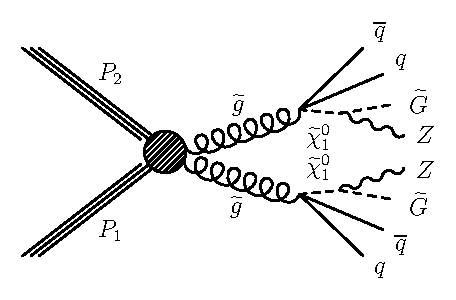
\includegraphics[width=0.4\textwidth]{intro/Feynman_graph_T5ZZgmsb.pdf} &
      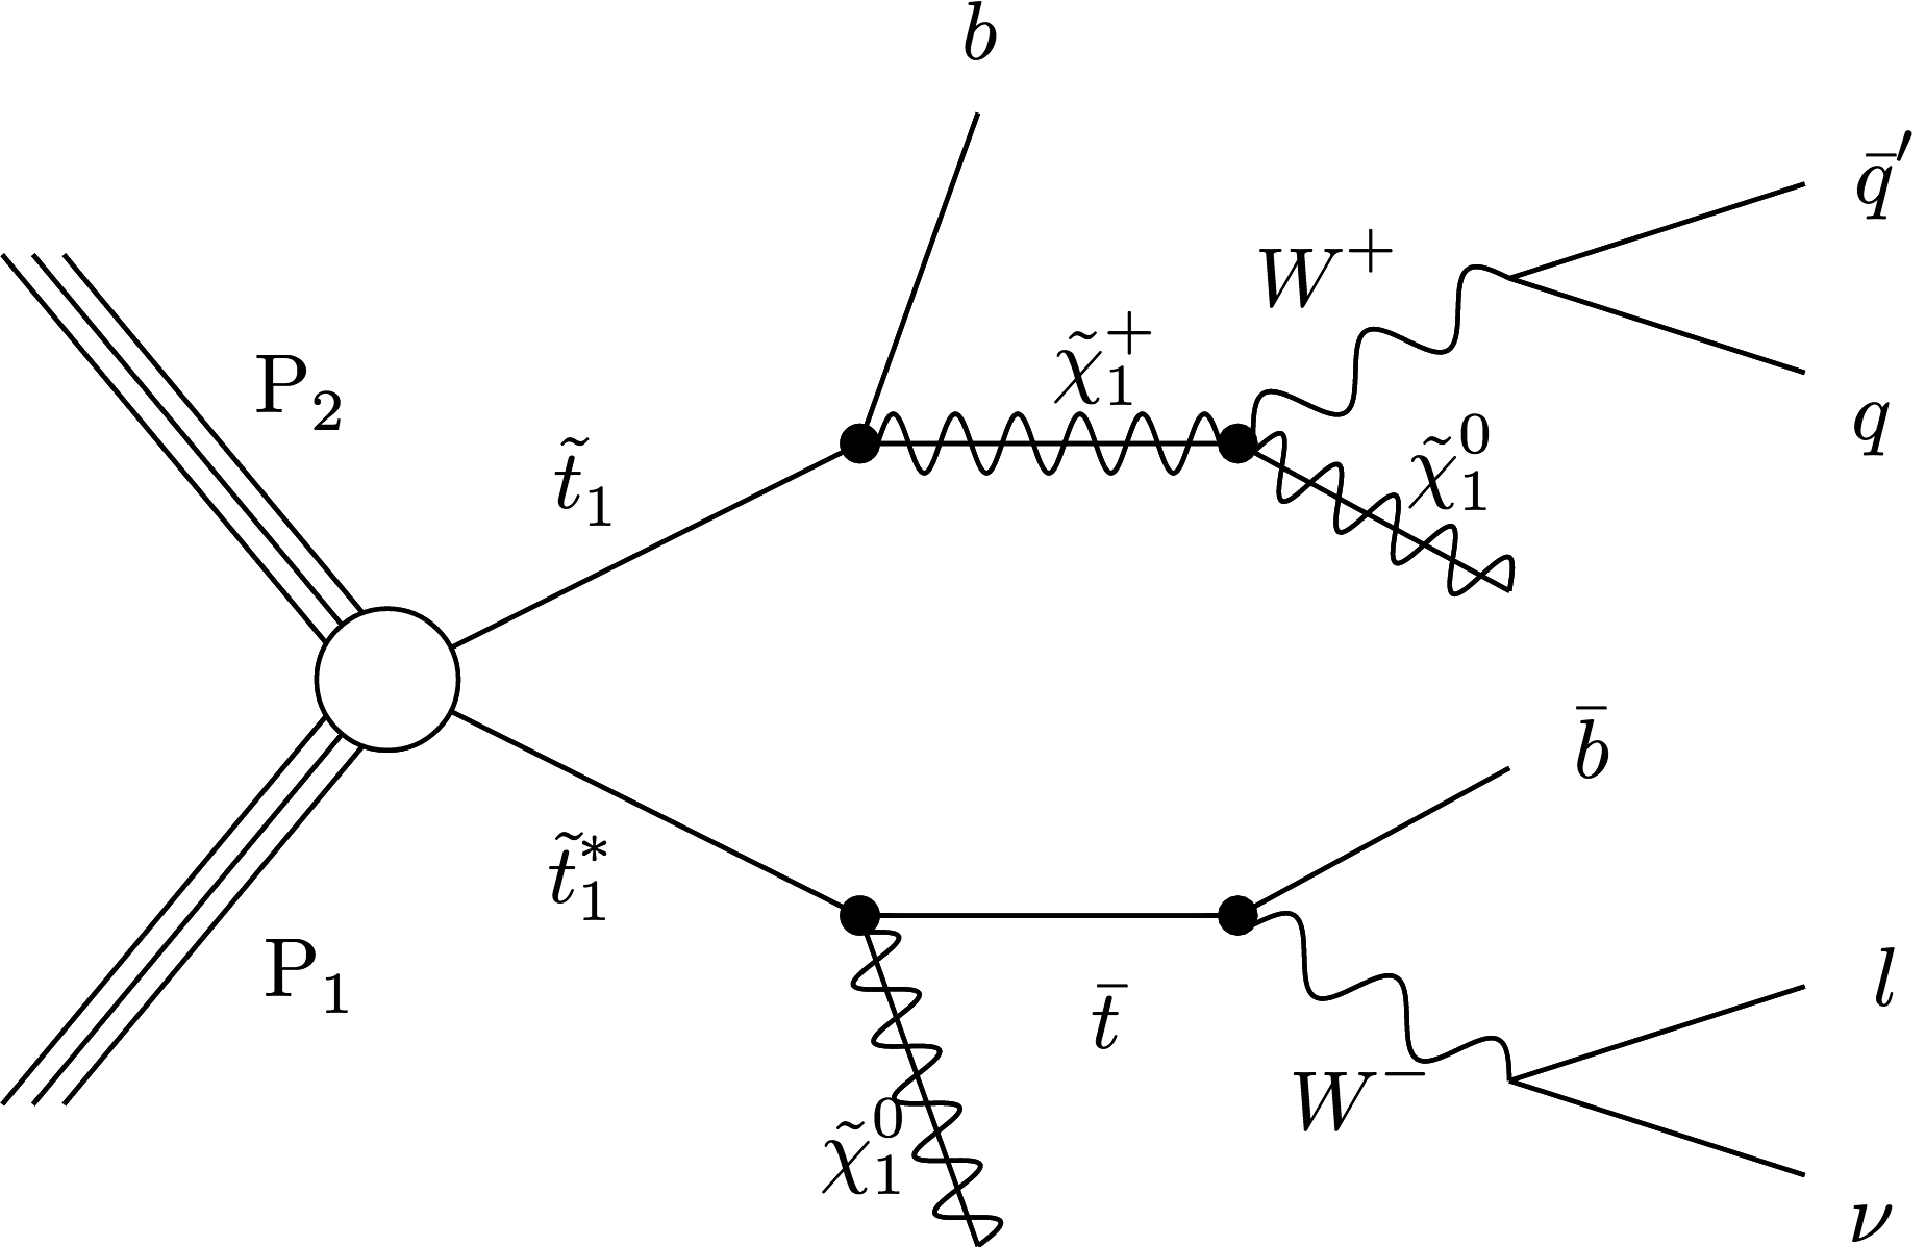
\includegraphics[width=0.4\textwidth]{intro/T2tt.pdf}
    \end{tabular}
    \caption{
      \label{fig:SMS_T5ZZgmsb}
      Diagrams showing different SUSY processes which may contain leptons in the final state are shown in this figure.
      On the left, gravitinos are pair-produced, where each eventually decays to a Z boson, two quarks, and a gravitino.
      On the right, stops are pair-produced, where one leg eventually decays to a top and a neutralino where the top decays leptonically.
    }
  \end{center}
\end{figure}

The SUSY analyses performed by CMS target a large range of topologies with varying
visible energy ($\mathrm{H_T,~M_J}$), 
invisible energy (\MET,
$\mathrm{M_T}$,
$\mathrm{M_{T2}}$,
$\mathrm{d\phi(\ell, W)}$,
$\mathrm{L_T}$),
jet multiplicity ($\mathrm{N_{jets}}$)
and flavor content ($\mathrm{N_{b-tags}}$).
The analyses are grouped by the number of leptons in the final state,
and for analyses with at least two leptons,
they are categorized according to the charge of the two leptons with the highest \pt
in same-sign, or opposite-sign final states.


In the analyses with exactly one lepton, three separate searches are performed.
In the first search, a search for direct stop pair production, the signal region is defined by having
exactly 1 lepton, njets, btags, and large MET.
After these cuts are made, the largest background comes from SM ttbar to dilepton, where one of the leptons is lost, leading to increased \MET.
The results of this analysis increase the sensitivity to stop production for signal models with a stop mass of 750 GeV,
which is an improvement on the previous result which was sensitive to models with a stop mass up to 650 GeV.
%% of the analysis done using data with pp collisions having an 8 TeV center of mass energy.

The next analysis is a search targeting final states with exactly one lepton, and many jets from hadronic top decay.

The final analysis with exactly one lepton, uses the dphi met W variable to discriminate background from signal.


The rest of the analyses all require at least 2 leptons in the final state.
The first analysis in this category is a search for SUSY in a final state with two same sign leptons.
This analysis is an inclusive search designed to be sensitive to many SUSY scenarios.
The baseline selection requires at least two same sign leptons with \pt\ $>$ 10-15 GeV depending on the trigger.

\begin{figure}[!htb]
\begin{center}
\begin{tabular}{cc}
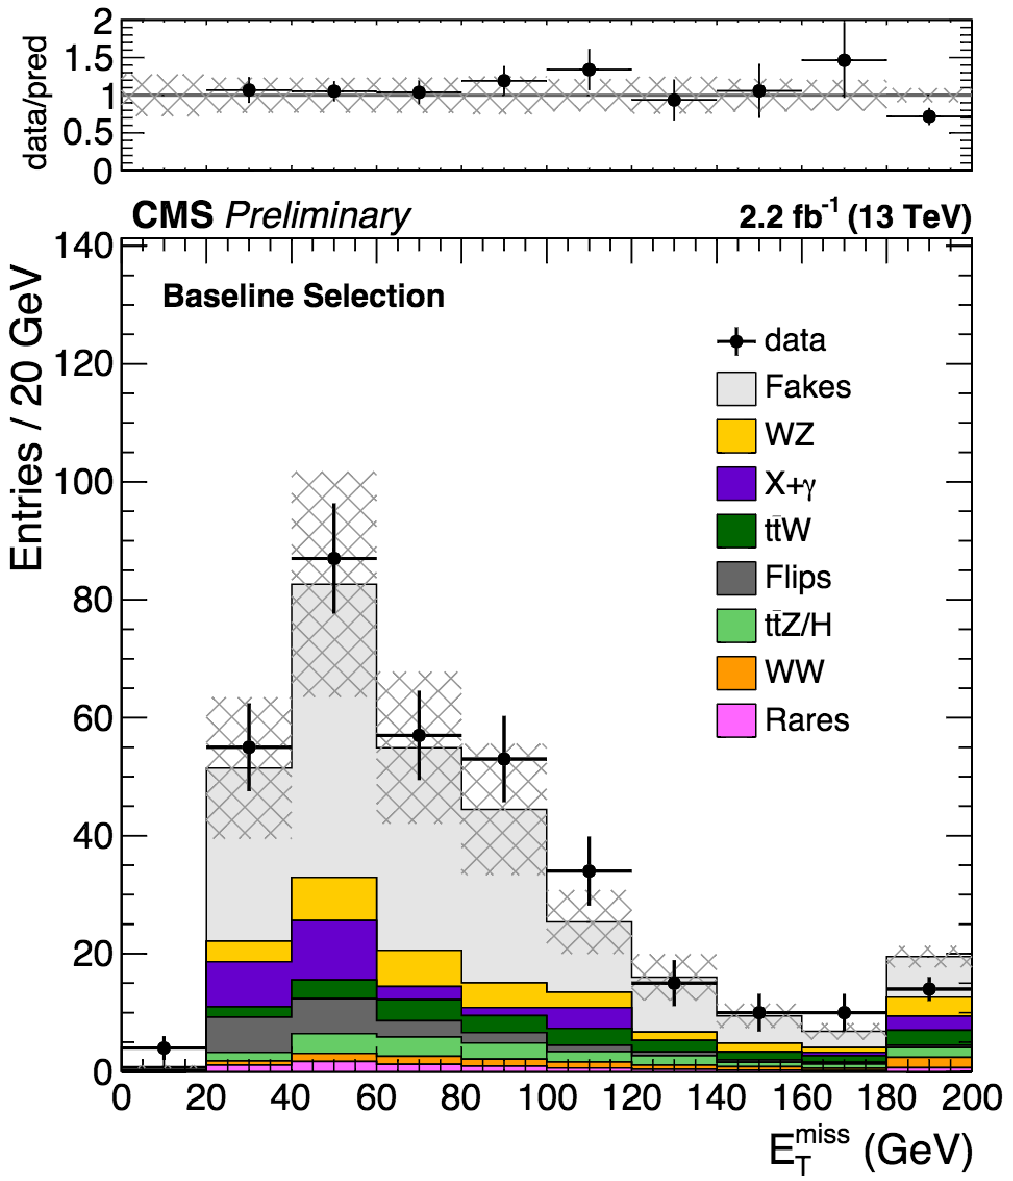
\includegraphics[width=0.4\textwidth]{2lepss/SS_MET.pdf} &
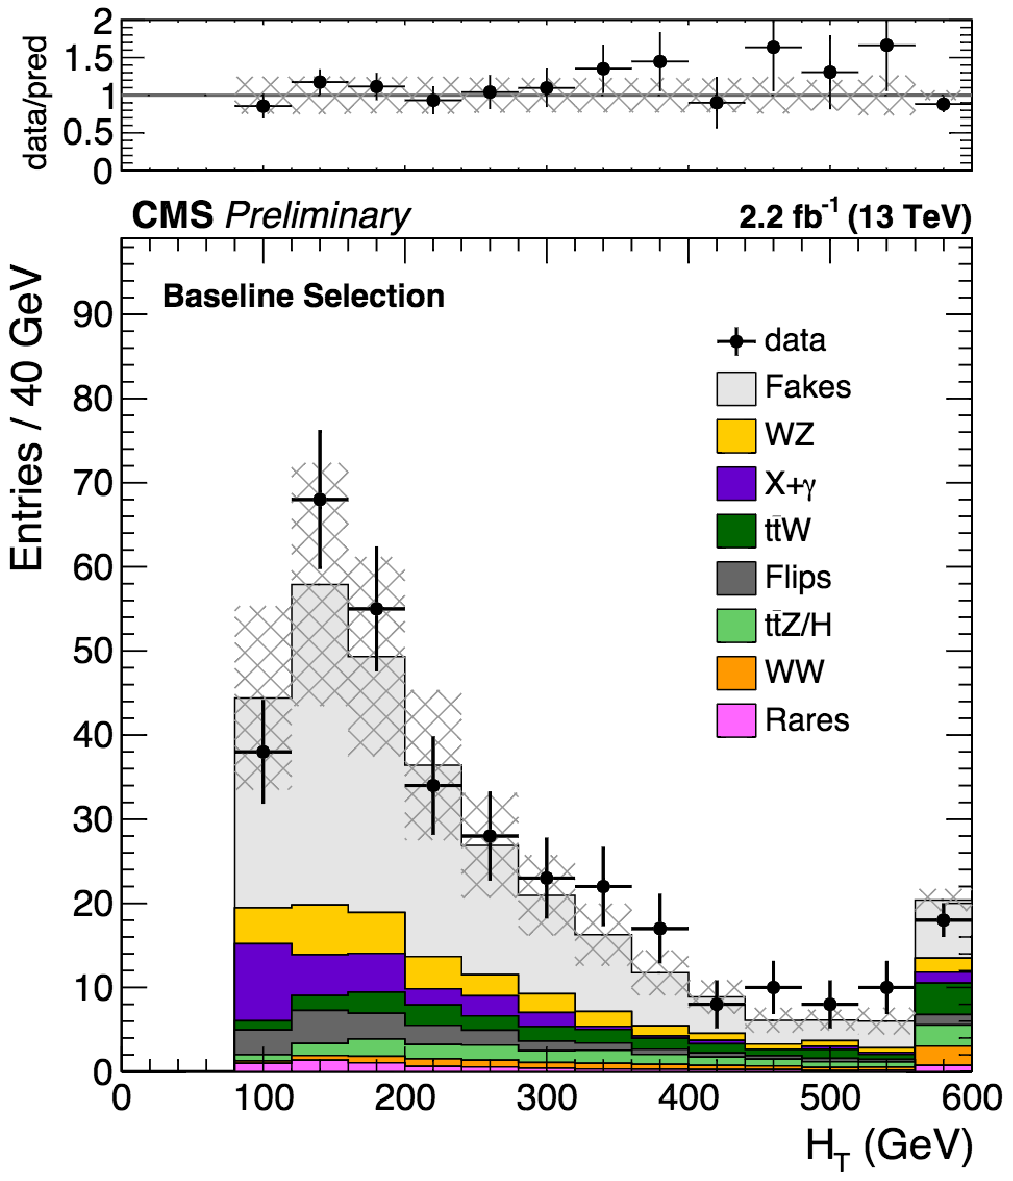
\includegraphics[width=0.4\textwidth]{2lepss/SS_HT.pdf}
\end{tabular}
\caption{
\label{fig:2lepssresults}
Observed yields and background predictions are shown for the same-sign dilepton analysis
for the variables \MET\ (left) and \HT\ (right).
}
\end{center}
\end{figure}


The next analysis is a search in events with three or more leptons.

The final analysis is a search in final states with at least two opposite-sign same-flavor leptons.
In this final state, two separate excesses were seen in run I.
CMS saw an excess in events with Mll 20-70 GeV with a significance of 2.6 sigma where ATLAS saw no excess,
and ATLAS observed a 3 sigma excess in events with two leptons with Mll 81-101, at least large HT, and large MET,
and the result from CMS in a similar signal region showed no significant deviation from the SM prediction.




Conclusion



% BibTeX users please use 
\bibdata{refs}
\bibliographystyle{ieeetr.bst}
\bibliography{refs}

%

%% % Non-BibTeX users please use
%% \begin{thebibliography}{}
%% %
%% % and use \bibitem to create references.
%% %
%% \bibitem{mycitation}
%% % Format for Journal Reference
%% Journal Author, Journal \textbf{Volume}, page numbers (year)
%% % Format for books
%% \bibitem{othercitation}
%% Book Author, \textit{Book title} (Publisher, place, year) page numbers
%% % etc
%% \end{thebibliography}
\end{document}
